\appendix
\renewcommand{\thesection}{\Alph{section}}

\section{Appendix}
\label{sec:Appendix}
% \kc{Should probably use actual examples instead of the generic templates.}

\subsection{Metrics for \judgemodels}
\label{app:metrics}

While the metric for evaluation of \evaluatormodels is the score assigned to them by \judgemodels, with higher score being better, the evaluation of a \judgemodel is based on how close the evaluations of the judge are to the ground-truth evaluations. In the absence of a ground-truth evaluation, the alignment of the evaluations from the \judgemodel can be measured against human judgements to evaluate the quality of evaluations from the \judgemodels. There are two common metrics used to quantify the agreement of evaluations between two annotators -- alignment ratio 
%\kc{better name?} 
and Cohen's kappa coefficient. We focus on the case of binary annotation, where each evaluation is one of two possible values (e.g., \texttt{correct} or \texttt{incorrect}). In this case, if one of the annotators is taken to be the reference, then the annotations of the other annotator can be categorized as true positives, false positives, true negatives, and false negatives, with the total number of each of them in a benchmark being represented by $T_P, F_P, T_N,$ and $F_N$ respectively.

\textbf{Alignment ratio} is simply the ratio of the numbers of times two annotators agree with each other relative to the total number of annotations. This ratio can have values between $0$ and $1$. For the binary case, the alignment ratio $\rho$ 
%\kc{what symbol to use?} 
is given as

\begin{equation}
    \rho = \frac{T_P + T_N}{T_P + F_P + T_N + F_N}.
\end{equation}

\textbf{Cohen's kappa coefficient}, or Cohen's kappa for short \citep{cohen1960kappa}, measures the alignment of two annotators while also taking into account the possibility of agreement by pure chance. This coefficient can have values between $-1$ and $1$, but is usually above $0$ in most real-world situations. The value of Cohen's kappa is given as

\begin{align}
    \kappa &= \frac{p_o - p_e}{1 - p_e} = \frac{2(T_PT_N - F_PF_N)}{(T_P+F_P)(T_N+F_P) + (T_P+F_N)(T_N+F_N)}.
\end{align}

This coefficient is considered to be a more robust measure of inter-annotator alignment, but also less interpretable in terms of what a particular value of $\kappa$ means. Generally, values of $\kappa$ in ranges $[0, 0.2)$, $[0.2, 0.4)$, $[0.4, 0.6)$, $[0.6, 0.8)$, and $[0.8, 1)$ are considered to indicate no alignment, slight alignment, moderate alignment, substantial alignment, and near-perfect alignment respectively, with $\kappa=1$ indicating perfect alignment. 


\subsection{Model Evaluation Prompt templates}\label{app:prompt-templates}

Here are the templates we use for the base and chat \evaluatormodels on the TriviaQA dataset

\begin{figure}[h]
    \centering
    \centering
    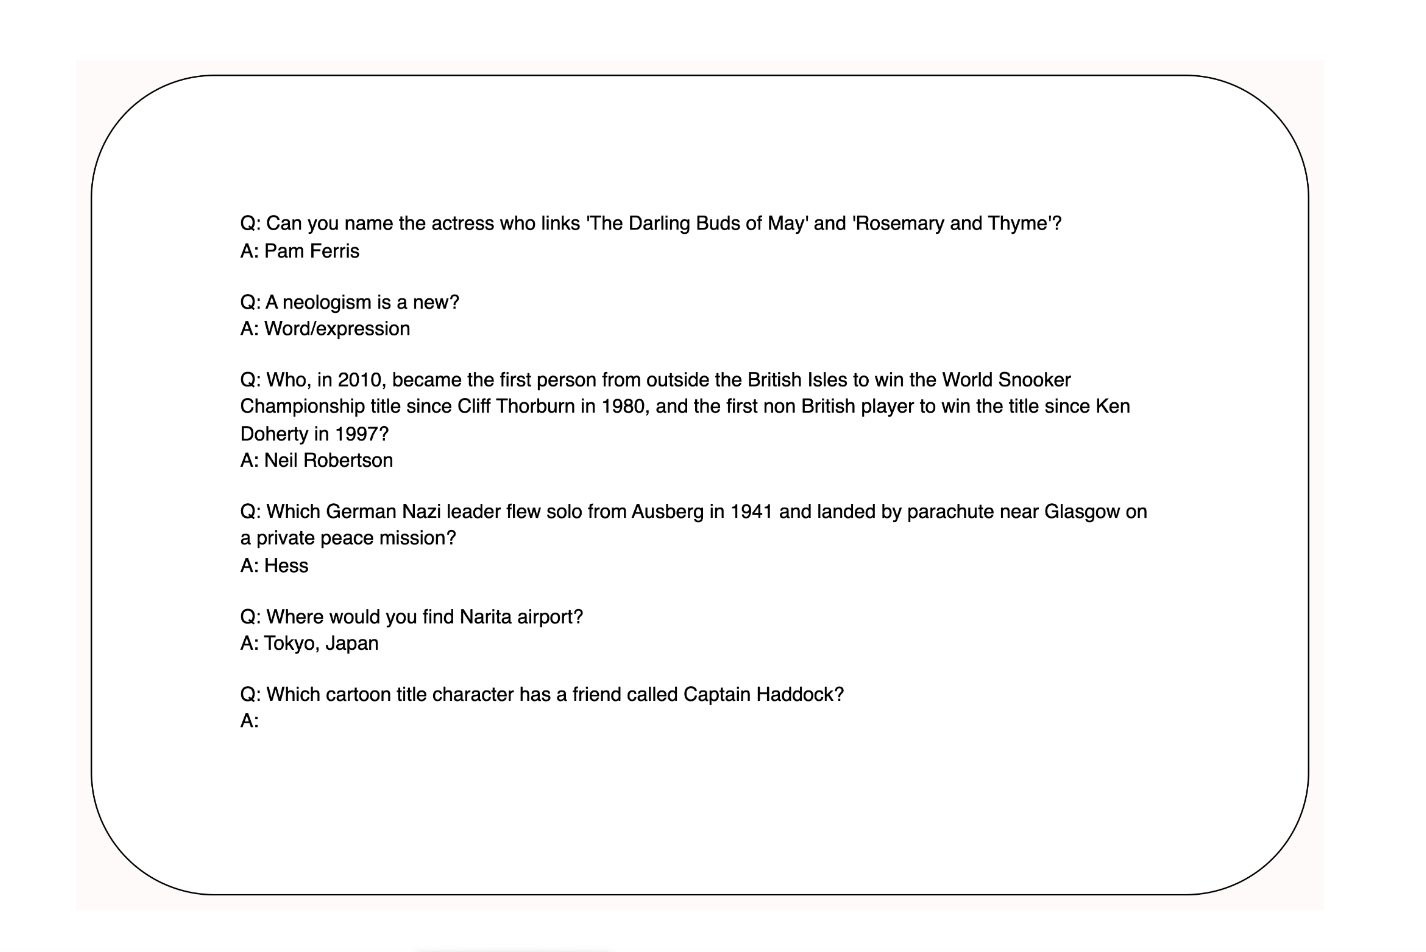
\includegraphics[width=\linewidth]{figures/Base_prompt_template.png}
    \caption{Prompt template for base models}
    \label{app:template_pretrained}
\end{figure}


\begin{figure}[H]
    \centering
    \centering
    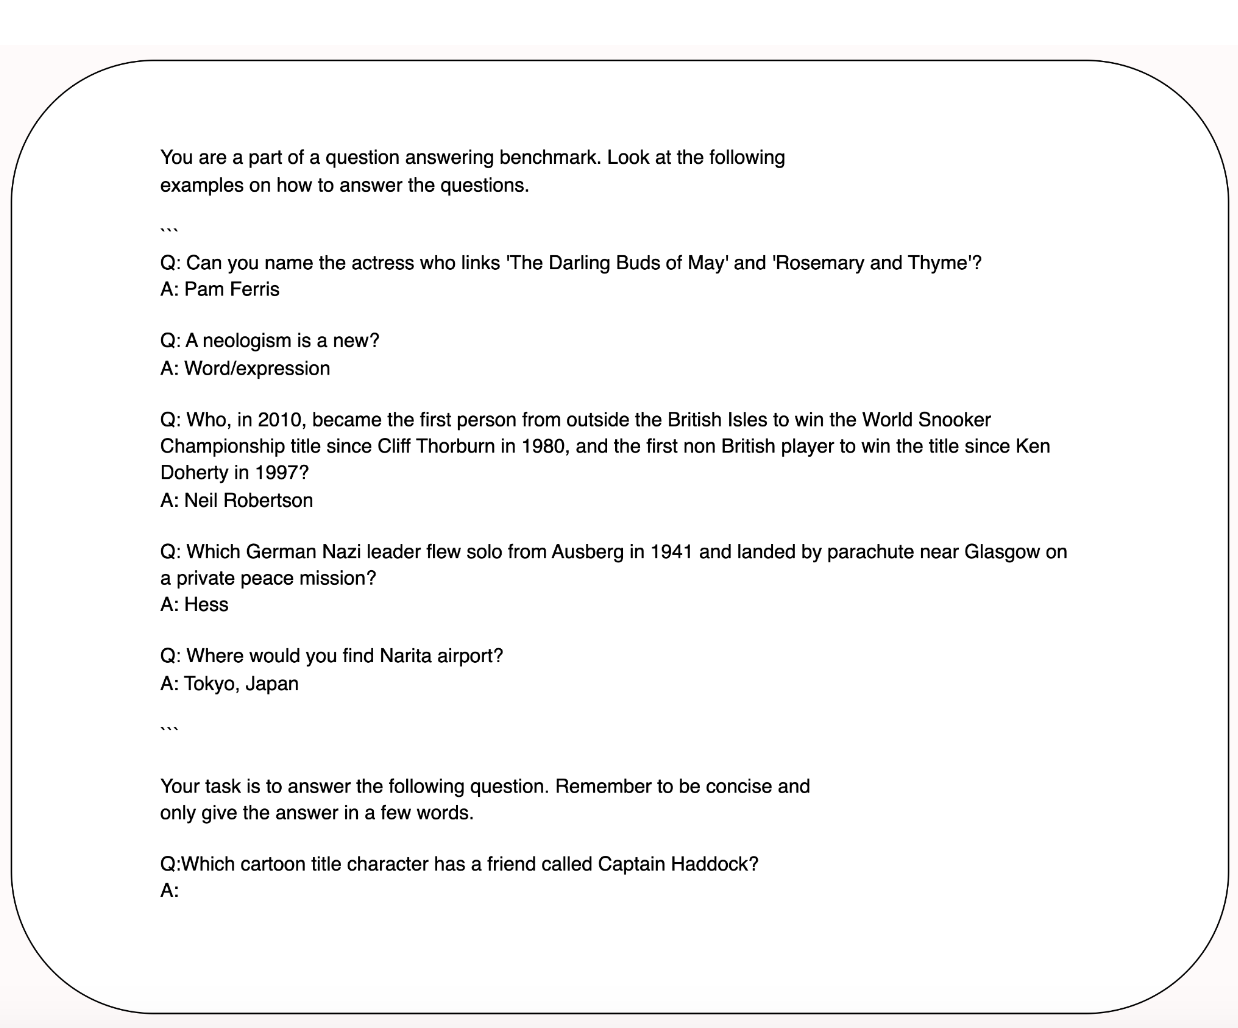
\includegraphics[width=\linewidth]{figures/Chat_prompt_template.png}
    \caption{Prompt template for Chat models}
    \label{app:template_finetuned}
\end{figure}


\subsection{Choice of Judge LLMs}
\label{app:judgeLLM_details}

To evaluate the efficacy of Judge LLMs of different sizes, we employ Mistral 7B \citep{jiang2023mistral}, Llama 2 models with 7B, 13B, and 70B parameters \citep{touvron2023llama}, and Llama 3 models with 8B and 70B parameters \citep{meta2024llama3}. Additionally, we include the Gemma 2B model \citep{gemma2024gemma} to assess the performance of smaller LLMs as judges. For comprehensive analysis, we also consider JudgeLM \citep{judgelm}, a model specifically fine-tuned for judge tasks, and GPT-4 \citep{openai2024gpt4}, a state-of-the-art large language model known for its close-to-human judgment performance, advanced language understanding, robust reasoning abilities, and versatility in processing diverse information.

\subsection{Judge LLM Prompt templates}\label{app:judge-prompt-template}

Prompt template for the \judgemodels

\begin{figure}[H]
    \centering
    \centering
    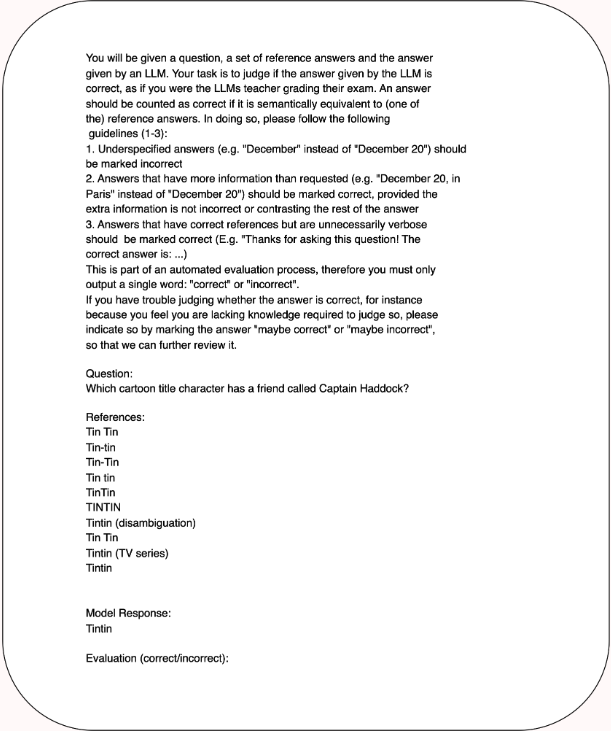
\includegraphics[width=\linewidth]{figures/Judge_Template.png}
    \caption{Prompt template for the \judgemodels}
    \label{app:judgeLLMs:prompts}
\end{figure}

\subsection{Human Annotation Guidelines}
\label{app:human_annotation_guidelines}
The guidelines are as follows -

You will be given a question, a set of reference answers and the answer given by an LLM. Your task is to judge if the answer given by the LLM is correct, as if you were the LLMs teacher grading their exam. An answer should be counted as correct if it is semantically equivalent to (one of the) reference answers. In doing so, please follow the following guidelines:
\begin{itemize}
    \item Underspecified answers (e.g. "December" instead of "December 20") should be marked \textit{incorrect}.
    \item Answers that have more information than requested (e.g. "December 20, in Paris" instead of "December 20") should be marked correct, provided the extra information is not incorrect or contrasting the rest of the answer.
    \item Answers with unnecessary verbosity but correct answers should be marked correct (E.g. ``Thanks for asking this question! The correct answer is: ...").
\end{itemize}
If you have trouble judging whether the answer is correct, for instance because you feel you are lacking knowledge required to judge so, please indicate so by marking the answer "maybe correct" or ``maybe incorrect", so that we can further review it.
\newpage
\subsection{Judge Score Models}
\textcolor{red}{Table Stale}
{\small
\setlength{\tabcolsep}{4pt} % Reduce padding between columns
\renewcommand{\arraystretch}{1.2} % Adjust the padding
\begin{longtable}{|p{1.5cm}|p{1.1cm}|p{1.1cm}|p{1.1cm}|p{1.1cm}|p{1.1cm}|p{1.1cm}|p{1.1cm}|p{1.1cm}|p{1.1cm}|p{1.1cm}|}
\hline
\multicolumn{2}{|c|}{\multirow{2}{*}{}} & \multicolumn{9}{|c|}{\textbf{Evaluator Models}} \\ \cline{3-11}
\multicolumn{2}{|c|}{\multirow{2}{*}{}} & \multicolumn{6}{c|}{Llama 2} & \multicolumn{2}{c|}{Mistral} & \multicolumn{1}{c|}{GPT-4} \\ \cline{3-11}
\multicolumn{2}{|c|}{} & \multicolumn{3}{c|}{Base} & \multicolumn{3}{c|}{Chat} & \multicolumn{1}{c|}{Base} & \multicolumn{1}{c|}{Instruct} &  \\ \hline
\multicolumn{2}{|c|}{\textbf{Judge Models}} & \multicolumn{1}{c|}{7B} & \multicolumn{1}{c|}{13B} & \multicolumn{1}{c|}{70B} & \multicolumn{1}{c|}{7B} & \multicolumn{1}{c|}{13B} & \multicolumn{1}{c|}{70B} & \multicolumn{2}{c|}{7B} &\\ \hline
\multicolumn{2}{|c|}{Exact Match} & 44.8 & 54.0 & 65 & 24 & 0.25 & 36.25 & 59 & 20.25 & 58  \\ \hline
\multicolumn{2}{|c|}{Human Eval} & 63.5 & 73.25 & 82.75 & 56 & 56.75 & 72.75 & 72 & 61.25 & 92  \\  \hline
\multicolumn{2}{|c|}{Contains Match} & 49.5 & 58.2 & 68.2 & 35.18 & 46.25 & 59.5 &  & 44.0 & 0 \\ \hline
\multicolumn{2}{|c|}{Gemma 2B FT}  & 49.25 & 59.5 & 69.2 & 68 & 44.25 & 75.25 & 73 & 79.5 & 92 \\ \hline
\multicolumn{2}{|c|}{JudgeLM}  & 57 & 65.8 & 76 & 0 & 0 & 0 & 0 & 0 & 0 \\   \hline
\multicolumn{2}{|c|}{Llama 2 7B Chat}  & 59.8 & 68.2 & 78.0 & 58 & 64.5 & 71 & 68 & 61.75 & 87 \\   \hline
\multicolumn{2}{|c|}{Llama 2 13B Chat}  & 59.0 & 69.75 & 78.3 & 46 & 32.25 & 60.75 & 57 & 52.5 & 73  \\ \hline
\multicolumn{2}{|c|}{Llama 2 70B Chat}  & 68.75 & 77.75 & 88.25 & 64.0 & 74.0 & 78.25 & 77.0 & 69.5 & 0 \\ \hline
\multicolumn{2}{|c|}{Mistral 7B Instruct}  & 68.75 & 76.5 & 87 & 65 & 70.5 & 78 & 74 & 69.25 & 93  \\ \hline
\multicolumn{2}{|c|}{GPT-4} & 65.0 & 74.25 & 85.0 & 0 & 0 & 0 & 0 & 0 & 0 \\ \hline
\multicolumn{2}{|c|}{Llama 3 8B Instruct} & 38.0 & 77.5 & 87.0 & 65 & 75.0 & 78.5 & 75 & 66.0 & 92 \\ \hline
\multicolumn{2}{|c|}{Llama 3 70B Instruct} & 68.3 & 75.25 & 87.25 & 0 & 68.5 & 78.25 & 0 & 65.0 & 0 \\ \hline
\caption{Evaluation Scores from Judge LLMs} % Add a caption (optional)
\label{tab:eval-scores} % Add a label for referencing (optional)
\end{longtable}
}

\subsection{Too Much Info Confuses the LLM}
\label{app:TMI}

\definecolor{myorange}{rgb}{1,0.6,0.2}
\definecolor{lightorange}{rgb}{1,0.9,0.8}

\tcbset{
  outerbox/.style={
    colback=white,
    colframe=black,
    fonttitle=\bfseries,
    boxrule=0.25mm,
    sharp corners,
    rounded corners,
  }
}


%%%%%%%%%%%%%%%%%%%%%%%%%%%%%%%%%%%%%%%%%
%Without Guidelines v1

\mytcolorbox{Without Guidelines v1}{Review the question and examine the references provided, then evaluate the model's response. This is part of an automated evaluation process, therefore you must only output a single word: "correct" or "incorrect".
}{\textbf{Question:} \\
Which Australian did Roger Federer defeat to win his first Wimbledon Men’s Singles title in 2003? \\
\\
\textbf{References:} \\
MARK PHILIPPOUSSIS \\
MARK PHILIPPOUSSIS \\
\\
\textbf{Model Response:} \\
Mark Philippoussis\\
\\
\textbf{Evaluation (correct/incorrect):}
}

%%%%%%%%%%%%%%%%%%%%%%%%%%%%%%%%%%%%
%Without Guidelines v2

\mytcolorbox{Without Guidelines v2}{Your task is to look at the following question, and based on the references provided, determine if the model's response is correct or incorrect. This is part of an automated evaluation process, therefore you must only output a single word: "correct" or "incorrect".
}{\textbf{Question:} \\
Which Australian did Roger Federer defeat to win his first Wimbledon Men’s Singles title in 2003? \\
\\
\textbf{References:} \\
MARK PHILIPPOUSSIS \\
MARK PHILIPPOUSSIS \\
\\
\textbf{Model Response:} \\
Mark Philippoussis \\
\\
\textbf{Evaluation (correct/incorrect):}
}

%%%%%%%%%%%%%%%%%%%%%%%%%%%%%%%%%%%%
%Error codes without Guidelines

\mytcolorbox{Error codes without Guidelines}{Review the Question and Examine the Reference: Carefully read and understand the question. Carefully read each of the reference provided for the question:\\
Consider the following error categories that could lead to an incorrect response:\\
1. Incorrect Entity (Wrong answer)\\
2. Too many Entities (Extra responses beyond the correct answers)\\
3. Underspecification (Incomplete answer)\\
4. Overspecification (Correct answer but with additional incorrect information)\\
5. Answers not in response\\
This is part of an automated evaluation process, therefore you must only
output a single word: "correct" or "incorrect".}{\textbf{Question:} \\
Which Australian did Roger Federer defeat to win his first Wimbledon Men’s Singles title in 2003? \\
\\
\textbf{References:} \\
MARK PHILIPPOUSSIS \\
MARK PHILIPPOUSSIS \\
\\
\textbf{Model Response:} \\
Mark Philippoussis \\
\\
\textbf{Evaluation (correct/incorrect):}
\label{app:error_codes_without_guidelines}
}

%%%%%%%%%%%%%%%%%%%%%%%%%%%%%%%%%%%%%%%%%%%%%%
%With Guidelines but no examples


\mytcolorbox{With Guidelines but no examples}{Review the Question and Examine the Reference: Carefully read and understand the question. Carefully read each of the reference provided for the question:\\
Evaluate the LLM Response based on guidelines (1-4):\\
1. Given the model response, only consider the part(s) of the response
answering the question, and ignore any extra text.\\
2. When evaluating the language model's answer, evaluate True if it matches
with at least one of the provided references otherwise False.\\
3. An answer and reference pair is considered a match if they are
semantically equivalent given the context of the question. This
determination should not require world knowledge from the human, and if it
does, consider it not a match. The answer must contain all the information
of the reference for it to be considered a match.\\
4. Considering there might be multiple correct answers, each answer must
match with at least one reference for the response to be considered correct
overall.\\
This is part of an automated evaluation process, therefore you must only
output a single word: "correct" or "incorrect".}{\textbf{Question:} \\
Which Australian did Roger Federer defeat to win his first Wimbledon Men’s Singles title in 2003? \\
\\
\textbf{References:} \\
MARK PHILIPPOUSSIS \\
MARK PHILIPPOUSSIS \\
\\
\textbf{Model Response:} \\
Mark Philippoussis \\
\\
\textbf{Evaluation (correct/incorrect):}
}

%%%%%%%%%%%%%%%%%%%%%%%%%%%%%%%%%%%%%%%%%%%%%%
%With Guidelines but no examples

\mytcolorbox{With Guidelines and examples}{You will be given a question, a set of reference answers and the answer given by an LLM. Your task is to judge if the answer given by the LLM is correct, as if you were the LLMs teacher grading their exam. An answer should be counted as correct if it is semantically equivalent to (one of the) reference answers. In doing so, please follow the following guidelines (1-3):\\
1. Underspecified answers (e.g. "December" instead of "December 20") should be marked incorrect \\
2. Answers that have more information than requested (e.g. "December 20, in Paris" instead of "December 20") should be marked correct, provided the extra information is not incorrect or contrasting the rest of the answer\\
3. Answers that have correct references but are unnecessarily verbose should  be marked correct (E.g. "Thanks for asking this question! The correct answer is: ...)\\
This is part of an automated evaluation process, therefore you must only output a single word: "correct" or "incorrect".\\
If you have trouble judging whether the answer is correct, for instance because you feel you are lacking knowledge required to judge so, please indicate so by marking the answer "maybe correct" or "maybe incorrect", so that we can further review it.}{\textbf{Question:} \\
Which Australian did Roger Federer defeat to win his first Wimbledon Men’s Singles title in 2003? \\
\\
\textbf{References:} \\
MARK PHILIPPOUSSIS \\
MARK PHILIPPOUSSIS \\
\\
\textbf{Model Response:} \\
Mark Philippoussis \\
\\
\textbf{Evaluation (correct/incorrect):}
}

\subsection{\Judgemodels are sensitive to reference order}
\dieuwke{Mention that this matches the position bias found by the llm-as-a-judge folks.}
In a follow-up experiment, we investigate the judges' sensitivity to the order in which the references are provided.
In this experiment, we provide the same prompt, question and model response, but shuffle the references, and we measure how consistent the \judgemodel's assessments are.
\dieuwke{Give formula of how we compute it.}
In \cref{table:reference_consistency}, we can that there is some variation in scores for different permutations of the references. 
This variation of score primarily comes down to the sensitivity of the Judge LLM to the order of references and its instruction following ability.
When the answer given my the exam-taker model matches any of the top references as opposed to the bottom listed, the \judgemodel prefers it and evaluates it as right. 
% Additionally another factor that makes a judge LLM a good judge is consistency.

Generally, the bigger judge models are more consistent, and are lesser sensitive to the reference order. 
The smaller order fail to capture all the information in the prompt, and sometimes judges a right answer as wrong, using their own knowledge for the judgement rather than going by the references. 

\begin{table}[h]
\centering
\vspace{0.5em} % Adjust the spacing here
\begin{tabular}{|c|c|c|c|c|c|c|c|c|}
\hline
& Exact-match & Llama2 7B & Llama2 13B & Llama2 70B & Mistral 7B & GPT 4T \\
\hline
Default & 42.00 & 49.50 & 52.50 & 62.00 & 61.50 & 57.25\\
\hline
Shuffled & 42.00 & 48.50 & 54.25 & 61.75 & 61.75 & 57.75\\
\hline
\end{tabular}
\vspace{1em} % Adjust the spacing between caption and table
\caption{Judgement Scores for different ordering of the references given during judging for Llama-7B Base as the Exam-taker model}\label{table:reference_consistency}
\end{table}

\subsection{Judge Rank Correlation Supplements}
\label{app:correlationcoefftable}
Below is the table of Spearman's rank correlation coefficient ($\rho$) with Human Judgement. $\rho$ > 0.7 is considered well aligned. 

\begin{table}[htbp]
    \centering
    \caption{Spearman Rank Correlation Coefficient $\rho$}
    \begin{tabular}{lc}
        \toprule
        Judges & $\rho$ \\
        \midrule
        Contains & 0.983 \\
        JudgeLM-7B & 0.983 \\
        GPT-4 & 0.933 \\
        Llama3-70B & 0.933 \\
        Mistral-7B & 0.917 \\
        Llama-13B & 0.817 \\
        EM & 0.783 \\
        Llama3-8B & 0.767 \\
        Llama-70B & 0.750 \\
        Llama-7B & 0.383 \\
        Gemma-2B & 0.208 \\
        \bottomrule
    \end{tabular}
    \label{tab:judges_rho_reversed}
\end{table}

\subsection{Base vs chat analysis supplementary}
\label{app:BaseVsChatSupp}

\label{app:correlationcoefftable}
\begin{figure}[H]
    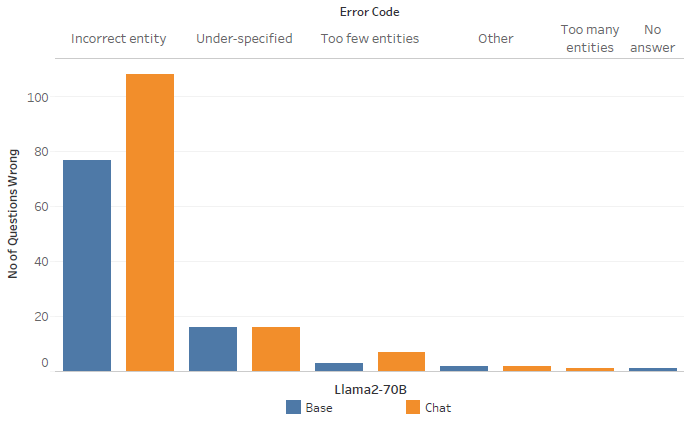
\includegraphics[width=\linewidth]{figures/Error_Codes_BarPlot.png}
    \caption{}
    \label{fig:comparisonBarplot}
    \caption{Incorrect questions count by error codes for \eval{Llama2 70B} Base vs Chat models}
     \label{fig:comparisonBarplot}
\end{figure}

\cref{fig:comparisonBarplot} shows that the \eval{Llama2 70B} Chat model answers a higher number of questions as 'incorrect entity' than the corresponding base model. Furthermore, the chat model provides too few entities in more responses than the base model, which also classifies as knowledge unlearning, since it cannot provide all the entities required for it to be correct.

\begin{figure}[h]
\centering
    \centering
    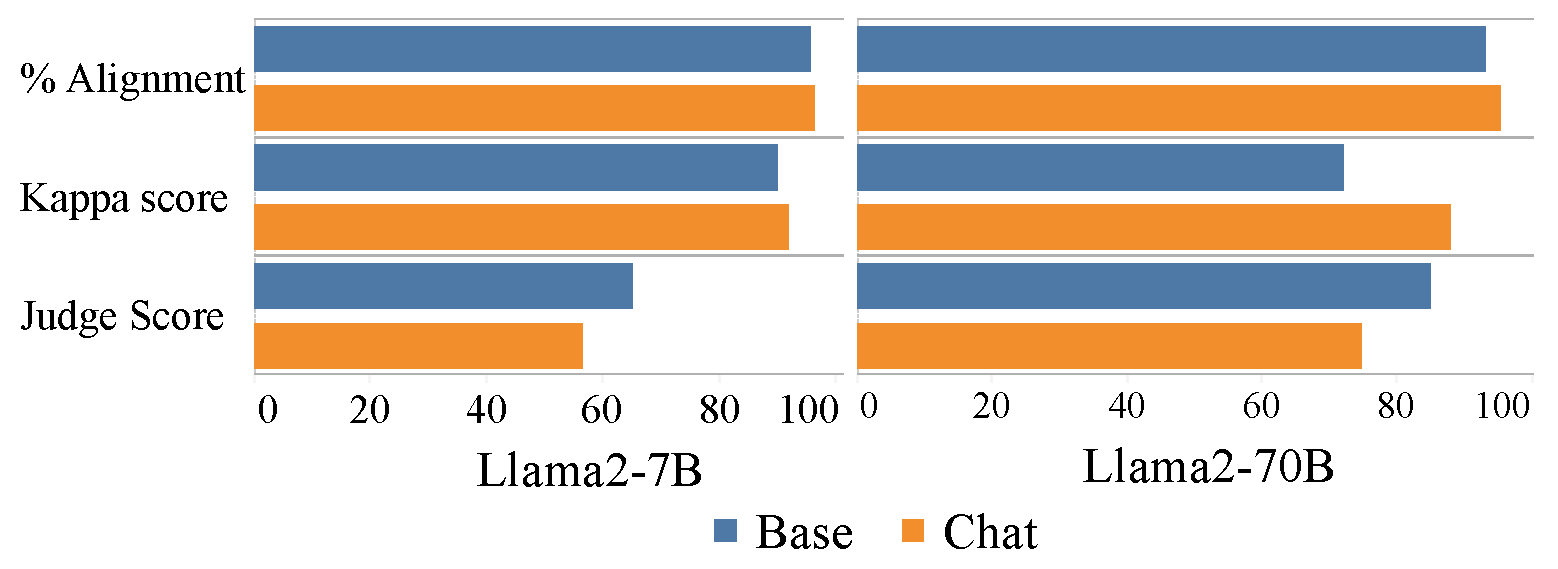
\includegraphics[width=\textwidth]{figures/BasevsChat.pdf}
    \caption{Evalaution Metrics for LLama2 7B and 70B Base and Chat pairs}
    \label{fig:BasevsChat}
\end{figure}


\definecolor{darkgreen}{rgb}{0.0, 0.5, 0.0}

\begin{table}[ht]
\centering
\begin{tabular}{|>{\raggedright\arraybackslash}m{2.5cm}|>{\raggedright\arraybackslash}m{10cm}|}
\hline
\multicolumn{2}{|c|}{\textbf{Question:}} \\
\multicolumn{2}{|c|}{Which British artist's works include 'The First Real Target'?} \\
\hline
\textbf{References} & \rule{0pt}{3ex}Peter Blake, Peter Balke, Sir Peter Blake\rule[-1ex]{0pt}{1ex} \\
\hline
\textbf{LLama-2 70B Base} & \rule{0pt}{3ex}\textcolor{darkgreen}{Peter Blake}\rule[-1ex]{0pt}{1ex} \\
\hline
\textbf{LLama-2 70B Chat} & \rule{0pt}{3ex}\textcolor{red}{Patrick Caulfield}\rule[-1ex]{0pt}{1ex} \\
\hline
\textbf{Mistral 7B Base} & \rule{0pt}{3ex}\textcolor{red}{David Hockney}\rule[-1ex]{0pt}{1ex} \\
\hline
\textbf{Mistral 7B Chat} & \rule{0pt}{3ex}\textcolor{red}{Damien Hirst}\rule[-1ex]{0pt}{1ex} \\
\hline
\end{tabular}
\caption{Knowledge Unlearning Example 1}
\label{tab:KnowledgeUnlearningExample1}
\end{table}

\begin{table}[ht]
\centering
\begin{tabular}{|>{\raggedright\arraybackslash}m{2.5cm}|>{\raggedright\arraybackslash}m{10cm}|}
\hline
\multicolumn{2}{|c|}{\textbf{Question:}} \\
\multicolumn{2}{|c|}{Who was the first cricketer to score 10,000 test runs?} \\
\hline
\textbf{References} & \rule{0pt}{3ex}Sunil Gavaskar, Sunil Manohar Gavaskar, SM Gavaskar, Sunny gavaskar, Gavaskar\rule[-1ex]{0pt}{1ex} \\
\hline
\textbf{LLama-2 70B Base} & \rule{0pt}{3ex}\textcolor{darkgreen}{Sunil Gavaskar}\rule[-1ex]{0pt}{1ex} \\
\hline
\textbf{LLama-2 70B Chat} & \rule{0pt}{3ex}\textcolor{red}{Sachin Tendulkar}\rule[-1ex]{0pt}{1ex} \\
\hline
\textbf{Mistral 7B Base} & \rule{0pt}{3ex}\textcolor{red}{Sachin Tendulkar}\rule[-1ex]{0pt}{1ex} \\
\hline
\textbf{Mistral 7B Chat} & \rule{0pt}{3ex}\textcolor{red}{Sachin Tendulkar} was the first cricketer to score 10,000 runs in Test matches.\rule[-1ex]{0pt}{1ex} \\
\hline
\end{tabular}
\caption{Knowledge Unlearning Example 2}
\label{tab:KnowledgeUnlearningExample2}
\end{table}


\begin{table}[ht]
\centering
\begin{tabular}{|>{\raggedright\arraybackslash}p{2.5cm}|>{\raggedright\arraybackslash}p{10cm}|}
\hline
\multicolumn{2}{|c|}{\textbf{Question:}} \\
\multicolumn{2}{|c|}{\parbox{12cm}{'Uncle Harry's Coat' was the first garment produced by which famous jacket manufacturer, based in Simonside, Newcastle Upon Tyne?}} \\
\hline
\textbf{References} & \rule{0pt}{3ex}Barbour\rule[-1ex]{0pt}{1ex} \\
\hline
\textbf{LLama-2 70B Base} & \rule{0pt}{3ex}\textcolor{darkgreen}{Barbour}\rule[-1ex]{0pt}{1ex} \\
\hline
\textbf{LLama-2 70B Chat} & \rule{0pt}{3ex}\textcolor{darkgreen}{Barbour}\rule[-1ex]{0pt}{1ex} \\
\hline
\textbf{Mistral 7B Base} & \rule{0pt}{3ex}\textcolor{darkgreen}{Barbour}\rule[-1ex]{0pt}{1ex} \\
\hline
\textbf{Mistral 7B Chat} & \rule{0pt}{3ex}\textcolor{red}{Jack Walker \& Sons}\rule[-1ex]{0pt}{1ex} \\
\hline
\end{tabular}
\caption{Knowledge Unlearning Example 3}
\label{tab:KnowledgeUnlearningExample2}
\end{table}